\documentclass{theme/uniprthesis}

%%%%%%%%%%%Some Extra Packages%%%%%%%%%%%
\usepackage[italian]{babel}		% To have Italina names in Sections, Figures, Chapters etc.
\usepackage{todonotes}			% To ease the revision

\usepackage{enumitem}
\usepackage{svg}
\usepackage{blindtext} 			% Dummy Text - remove
\usepackage{tikz}
\def\checkmark{\tikz\fill[scale=0.4](0,.35) -- (.25,0) -- (1,.7) -- (.25,.15) -- cycle;} 
\usepackage{ mathtools , amssymb , amsthm }

\usepackage{fancyvrb,fvextra}

\floatname{algorithm}{Codice}
%%%%%%%%%%%%%%%%%%%%%%%%%%%%%%%%%


%%%%% THESIS / TITLE PAGE INFORMATION
% Everybody needs to complete the following:

\title{LLM a progettazione di Lunar: \\ un linguaggio a dominio specifico \\ per giochi di carte collezionabili}
\author{Davide Donadio}
\advisor{Prof. Eleonora Iotti}
\college{Dipartimento di Scienze Matematiche, Fisiche e Informatiche}
\degree{Corso di Laurea Triennale in Informatica}
\degreeyears{2022--2023}


% Not mandatory fields
\newcommand{\subTitle}{LLM to design Lunar: a domain-specific language \\ for trading card games} %Subtitle, usually the english version of the title

%\newcommand{\advisorSecond}{Prof. Nome2 Cognome2} % For multiple (up to 4) advisors -- if this is not present then also the remaining ones are automatically omitted
%\newcommand{\advisorThird}{Dott. Nome3 Cognome3} % For multiple (up to 4) advisors -- if this is not present then also the remaining ones are automatically omitted
%\newcommand{\advisorFourth}{Dott. Nome4 Cognome4} % For multiple (up to 4) advisors

 %\newcommand{\coadvisor}{Prof. co-Nome co-Cognome}For multiple (up to 4) coadvisors -- if this is not present then also the remaining ones are automatically omitted
\newcommand{\coadvisorSecond}{Prof. co-Nome2 co-Cognome2} % For multiple (up to 4) coadvisors -- if this is not present then also the remaining ones are automatically omitted
%\newcommand{\coadvisorThird}{Dott. co-Nome3 co-Cognome3} % For multiple (up to 4) coadvisors -- if this is not present then also the remaining ones are automatically omitted
%\newcommand{\coadvisorFourth}{Dott. co-Nome4 co-Cognome4} % For multiple (up to 4) coadvisors


\begin{document}

\maketitle

%%%% La dedica
\newpage
\thispagestyle{empty}
\null\vspace{\stretch{1}}
\begin{flushright}
 	\textit{A te che sembrerà incomprensibile.} \\
	\textit{A te che sembrerà un gioco da ragazzi.} \\
  	\textit{A te che sarà il nuovo obiettivo da raggiungere.} \\
\end{flushright}
\vspace{\stretch{3}}\null
\newpage

%%%% Gli indici
\pagestyle{plain}
\pagenumbering{roman}
\tableofcontents
%
\listoffigures    %Commentare se non vi sono Immagini
\listofalgorithms %Commentare se non vi sono Algoritmi
\listoftables     %Commentare se non vi sono Tabelle
%
%
%
%%%% La prefazione
\chapter*{Sommario} %Se si cambia il Titolo cambiare anche la riga successiva così che appia corretto nell'indice

Questa tesi esplora l'interazione tra linguaggio naturale e giochi di carte collezionabili, focalizzandosi su \emph{Magic: The Gathering} come caso di studio. L'obiettivo è analizzare come in questi contesti diventi importante avere un linguaggio naturale ben strutturato e prevedibile. Il contributo principale riguarda l'applicazione di un Large Language Model per generare degli script per le carte. Attraverso questo approccio, si sono valutate le potenzialità e le limitazioni dei modelli di linguaggio avanzati nell'ambito de generazione script utilizzando un linguaggio a dominio specifico. Sono stati eseguiti diversi esperimenti ed i migliori risultati quantitativi e qualitativi si sono ottenuti con uno Small Language Model.
Grazie a questi esperimenti, sarà possibile formalizzare il linguaggio nella sua interezza e verrà reso disponibile lo Small Language Model per la generazione di script delle carte.
%
%%%% I Capitoli di Contenuto	
\pagestyle{fancy}
\chapter*{Introduzione}\label{chapter:introduction}
\addcontentsline{toc}{chapter}{Introduzione}

\pagenumbering{arabic} % Settaggio numerazione normale
Negli ultimi decenni, i giochi di carte collezionabili hanno registrato una significativa crescita, diventando un fenomeno culturale di rilevanza globale. In questo contesto, uno dei titoli più noti è \emph{Magic: The Gathering}.

Questo documento si propone di esplorare gli aspetti fondamentali di \textit{Magic: The Gathering}, considerandolo non solo come un gioco di carte, ma come un sistema complesso ricco di sfide strategiche e di interesse intellettuale. Attraverso un approccio che combina teoria dei trasformatori, elaborazione del linguaggio naturale e apprendimento automatico, ci si addentrerà nelle basi di \textit{Magic: The Gathering} e oltre, con l'obiettivo di ampliare la comprensione e l'applicazione del gioco.

Nel capitolo introduttivo, verrà fornita una panoramica delle basi teoriche e concettuali sottese a \textit{Magic: The Gathering}, offrendo un'orientamento per i lettori interessati. Saranno esaminati i principi di base del gioco, delineando i concetti chiave come la struttura di un turno e le zone di gioco. Inoltre, sarà discusso il ruolo del motore di regole all'interno del contesto della digitalizzazione di giochi da tavolo e di carte, con particolare attenzione al motore di regole noto come Forge.

Successivamente, verrà esaminato l'ambito dell'elaborazione del linguaggio naturale, con una panoramica sull'evoluzione degli algoritmi e sull'architettura dei trasformatori. Sarà introdotta anche la tematica dei Modelli di linguaggio, con una particolare attenzione alle loro applicazioni, incluse le potenziali implicazioni nella generazione di script per le carte di in un motore di regole. I linguaggi di scripting che verranno presi in esame sono ForgeScript e Lunar.

Il ruolo del linguaggio ForgeScript e della nuova proposta rappresentata da Lunar sarà analizzato in una sezione dedicata, evidenziandone le caratteristiche e l'implicazione nel processo di creazione e gestione degli effetti di gioco. 

Infine, verrà delineata la metodologia che guida l'esperimento condotto, con un focus alle fasi di addestramento dei Large Language Model. Attraverso l'impiego di tecniche avanzate e l'utilizzo di risorse di calcolo ad alte prestazioni, si mira a migliorare la generazione automatica degli script per le carte di \textit{Magic: The Gathering}, aprendo nuove prospettive nel campo dell'intelligenza artificiale applicata ai giochi.

Questo documento si propone di offrire una visione chiara e completa delle tematiche trattate, con l'obiettivo di fornire una risorsa informativa e di riferimento per coloro che sono interessati a esplorare il mondo di \emph{Magic: The Gathering} e dei Large Language Model.
\chapter{Regole del gioco}\label{chapter:background}

In questo capitolo, verrà presentata una panoramica delle basi teoriche e concettuali, in particolare sui giochi di carte collezionabili, soffermandosi su \emph{Magic: The Gathering}. Esploreremo le regole fondamentali che governano il gioco, suddividendole in concetti chiave e zone di gioco. Successivamente, verrà fornita un'introduzione su come leggere una carta di Magic, comprendendo le informazioni essenziali presenti su di essa. Inoltre, si esaminerà il concetto di motore di regole all'interno del contesto di Magic: The Gathering, con un focus particolare sul caso d'uso di Forge e il suo impatto nel giocare e comprendere il gioco.

\section{\textit{Magic The Gathering}}\label{sec:magic_the_gathering}
I giochi di carte collezionabili (GCC) sono un tipo di gioco di carte in cui i giocatori creano il proprio mazzo utilizzando una vasta gamma di carte disponibili, ognuna con caratteristiche e abilità uniche. Questi giochi combinano strategia, collezionismo e competizione, offrendo un'esperienza di gioco dinamica e coinvolgente. Tra i vari GCC, \emph{Magic: The Gathering} (anche detto semplicemente \emph{MtG} o \emph{Magic})  è il più longevo e popolare, lanciato nel 1993 da \emph{Wizards of the Coast} e creato dal matematico Richard Garfield.

\emph{Magic} è un gioco di strategia in cui due o più giocatori si sfidano utilizzando mazzi di carte personalizzati, con l'obiettivo di ridurre i punti vita dell'avversario a zero. Ogni giocatore inizia con un mazzo composto da almeno 60 carte, che possono essere di diversi tipi, tra cui creature, incantesimi, artefatti e terre.

Il gioco si svolge in turni, durante i quali i giocatori possono pescare carte, mettere in gioco terre, evocare creature e lanciare incantesimi o abilità. Le terre forniscono mana, la risorsa necessaria per giocare le altre carte. Ogni carta ha un costo di mana, indicato nell'angolo superiore destro, che rappresenta la quantità di mana necessaria per giocarla.

Le creature possono attaccare gli avversari o difendere il proprio giocatore dagli attacchi nemici. Ogni creatura ha due valori numerici: la forza, che indica la quantità di danno che può infliggere, e la costituzione, che indica la quantità di danno che può subire prima di essere distrutta.

Gli incantesimi e gli artefatti, invece, hanno effetti variabili che possono influenzare il campo di battaglia, le creature, i giocatori o altre carte in gioco. Questi effetti possono essere temporanei o permanenti, e possono avere un impatto significativo sull'andamento della partita.

\subsection{Come leggere una carta di \emph{Magic}}\label{subsec:mtg_cards}
Una carta di \emph{Magic} presenta diverse componenti chiave che forniscono informazioni sulle sue caratteristiche e funzioni. Di seguito è riportata una descrizione delle principali componenti di una carta, con l'immagine nella Figura \ref{fig:one} come esempio\footnote{ Sezione ``Part of a Card" delle regole comprensive \cite{mtg-comp-rules}}:



\begin{figure}[ht]
	\centering
        \begin{tikzpicture}
            \node[anchor=south west,inner sep=0] (image) at (0,0) {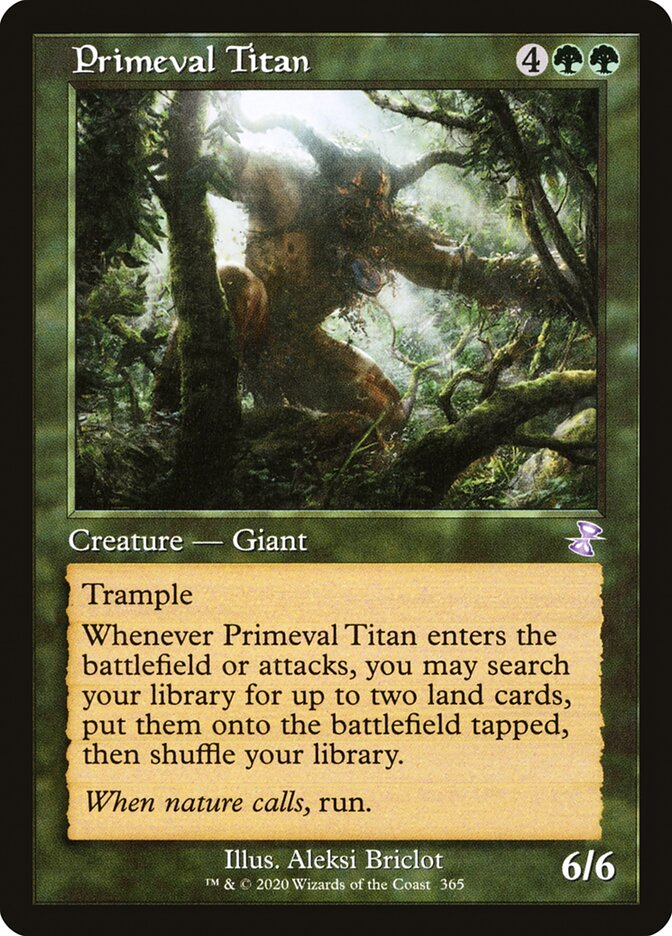
\includegraphics[width=0.5\textwidth]{Immagini/tsr-365-primeval-titan.jpg}};
            \begin{scope}[x={(image.south east)},y={(image.north west)}]
                \fill[red!50, opacity=0.5] (0.07,0.935) circle (0.27cm);
                \node [black, font=\Large] at (0.07,0.935) {a};
                \fill[red!50, opacity=0.5] (0.72, 0.94) circle (0.27cm);
                \node [black, font=\Large] at (0.72, 0.94) {b};
                \fill[red!50, opacity=0.5] (0.6, 0.6)  circle (0.27cm);
                \node [black, font=\Large] at (0.6, 0.6) {c};
                \fill[red!50, opacity=0.5] (0.07,0.42) circle (0.27cm);
                \node [black, font=\Large] at (0.07,0.42) {d};
                \fill[red!50, opacity=0.5] (0.5, 0.425)  circle (0.27cm);
                \node [black, font=\Large] at (0.5, 0.425) {e};
                \fill[red!50, opacity=0.5] (0.6, 0.15)  circle (0.27cm);
                \node [black, font=\Large] at (0.6, 0.15) {f};
                \fill[red!50, opacity=0.5] (0.25, 0.07)  circle (0.27cm);
                \node [black, font=\Large] at (0.25, 0.07) {g};
                \fill[red!50, opacity=0.5] (0.8, 0.07)  circle (0.27cm);
                \node [black, font=\Large] at (0.8, 0.07) {h};

            \end{scope}
        \end{tikzpicture}
	\caption{Carta di \emph{Magic the Gathering} con layout vintage}
	\label{fig:one}
\end{figure}




\begin{enumerate}[label=\alph*.]
    \item \textbf{Nome}: nella parte superiore della carta, si trova il nome univoco della carta, permettendo ai giocatori di identificarla facilmente e distinguerla dalle altre. 
    
    \item \textbf{Costo di mana}: nell'angolo superiore destro della carta, è presente il costo di mana necessario per giocare la carta, composto da simboli che rappresentano i diversi colori di mana (bianco, blu, nero, rosso e verde) e/o un numero che indica la quantità di mana generico richiesta.
    
    \item \textbf{Illustrazione}: al centro della carta, vi è un'illustrazione che rappresenta la carta e contribuisce all'ambientazione e all'atmosfera del gioco. 
    
    \item \textbf{Tipo di carta}: appena sotto l'illustrazione, si trova il tipo di carta, che può essere creatura, incantesimo, artefatto, terra, o una combinazione di questi. Il tipo di carta determina le regole generali che si applicano alla carta e il modo in cui può essere utilizzata durante il gioco. 
    
    \item \textbf{Sottotipo}: alcune carte hanno anche un sottotipo, che fornisce ulteriori informazioni sulla carta e sulle sue interazioni con altre carte. Ad esempio, una creatura potrebbe avere un sottotipo come ``Gigante" o ``Mago". 
    
    \item \textbf{Testo delle abilità}: nella parte centrale della carta, si trova il testo delle abilità, che descrive gli effetti e le regole specifiche della carta. Questo testo può includere parole chiave (Keywords), effetti che si attivano quando la carta entra in gioco, o abilità attivabili che richiedono un costo specifico per essere utilizzate. Può contenere anche un testo narrativo relativo al soggetto dell'illustrazione.
    
    \item \textbf{Informazioni legali e di collezionismo}: nella parte inferiore della carta, si trovano informazioni legali, il numero di collezionismo e l'edizione a cui appartiene la carta. Queste informazioni sono utili per i collezionisti e per determinare l'ammissibilità delle carte nei diversi formati di gioco. 
    
    \item \textbf{Forza/Costituzione}: per le carte creature, nella parte inferiore destra della carta, si trovano due numeri separati da una barra (/). Il primo numero indica la forza della creatura, ovvero la quantità di danno che può infliggere in combattimento\footnote{Questo argomento sarà approfondito nella Sezione \ref{subsec:mtg_turns} -- Parti del turno}, mentre il secondo numero rappresenta la costituzione, che indica la quantità di danno che la creatura può subire prima di essere distrutta.     
\end{enumerate}


\subsection{Le zone di gioco}\label{subsec:mtg_zones}
In \emph{Magic}, il tavolo di gioco si divide in diverse zone, ognuna delle quali ha uno scopo specifico e delle regole associate. Di seguito è riportata una descrizione delle principali zone di gioco\footnote{ Sezione ``Zones" delle regole comprensive \cite{mtg-comp-rules}}:


\begin{figure}[ht]
	\centering
        \begin{tikzpicture}
            \node[anchor=south west,inner sep=0] (image) at (0,0) {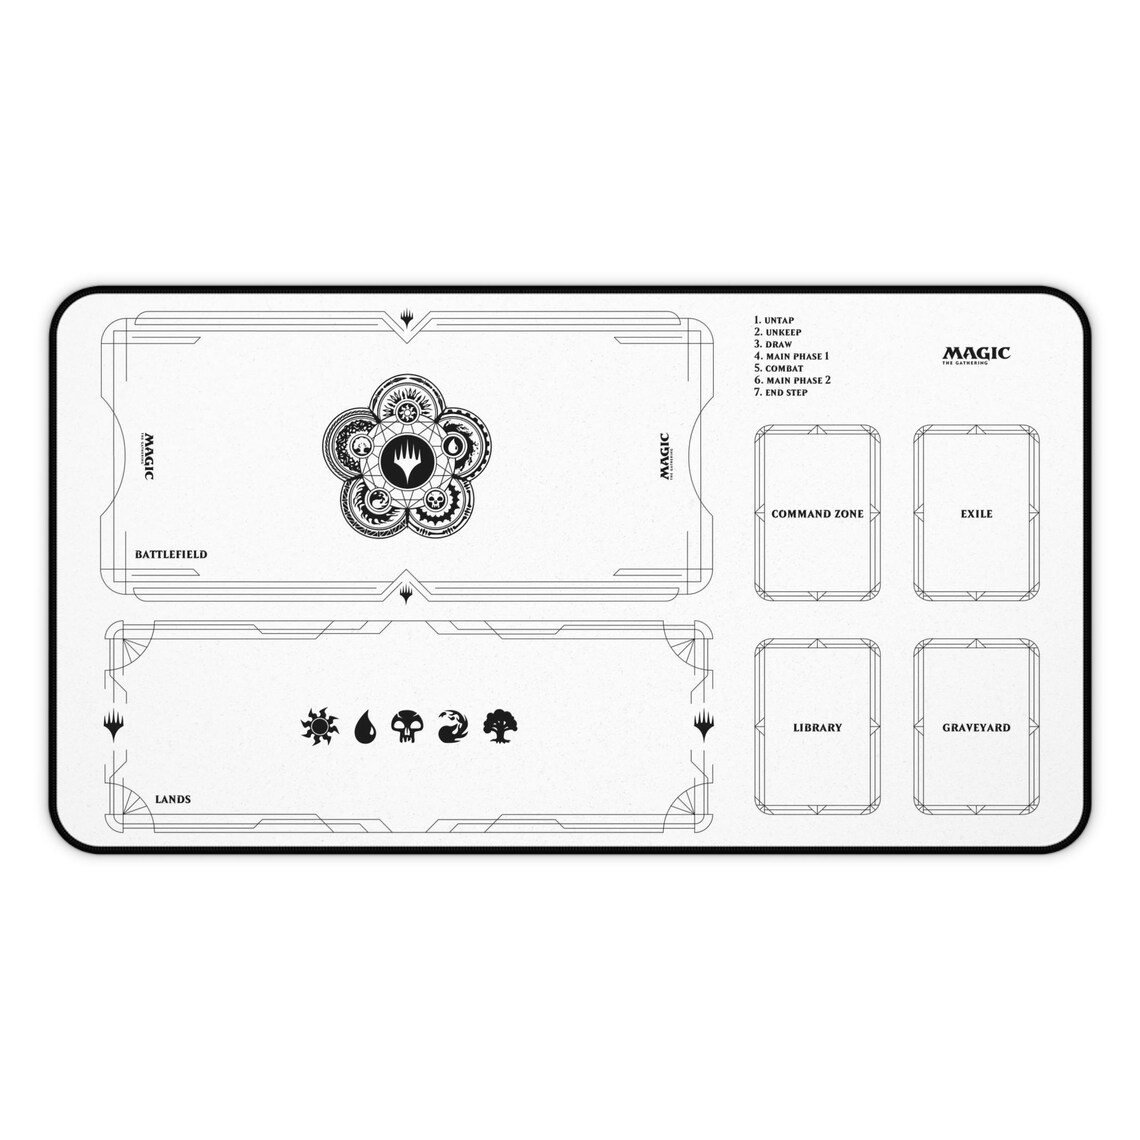
\includegraphics[width=\textwidth, trim= 0 200 0 200, clip]{Immagini/card_zones.jpg}};
            \begin{scope}[x={(image.south east)},y={(image.north west)}]
                \fill[red!50, opacity=0.5] (0.69,0.22) circle (0.27cm);
                \node [black, font=\Large] at (0.69,0.22) {a};
                \fill[red!50, opacity=0.5] (0.5, 0.07) circle (0.27cm);
                \node [black, font=\Large] at (0.5, 0.07) {b};
                \fill[red!50, opacity=0.5] (0.355,0.52) circle (0.27cm);
                \node [black, font=\Large] at (0.355,0.52) {c};
                \fill[red!50, opacity=0.5] (0.5, 0.92)  circle (0.27cm);
                \node [black, font=\Large] at (0.5, 0.92) {d};
                \fill[red!50, opacity=0.5] (0.825, 0.22)  circle (0.27cm);
                \node [black, font=\Large] at (0.825, 0.22) {e};
                \fill[red!50, opacity=0.5] (0.825, 0.5)  circle (0.27cm);
                \node [black, font=\Large] at (0.825, 0.5) {f};
                \fill[red!50, opacity=0.5] (0.69, 0.50)  circle (0.27cm);
                \node [black, font=\Large] at (0.69, 0.50) {g};

            \end{scope}
        \end{tikzpicture}
	\caption{Layout tipico del tavolo di gioco di \emph{Magic} (uno per giocatore)}
	\label{fig:two}
\end{figure}

\begin{enumerate}[label=\alph*.]
    \item \textbf{Grimorio (Library)}: Il grimorio è il mazzo di carte di un giocatore, disposto in un ordine casuale all'inizio della partita. I giocatori pescano carte dal loro grimorio durante il gioco. Non è consentito guardare le carte nel proprio grimorio o cambiarne l'ordine, a meno che una carta o un'abilità non lo consenta esplicitamente.
    
    \item \textbf{Mano (Hand)}: La mano di un giocatore è composta dalle carte che ha pescato ma non ha ancora giocato. I giocatori possono avere un massimo di sette carte in mano alla fine del loro turno, a meno che una carta o un'abilità non modifichi questo limite. Le carte in mano sono nascoste agli avversari.
    
    \item \textbf{Campo di battaglia (Battlefield)}: Il campo di battaglia è la zona di gioco in cui si trovano i permanenti, come creature, artefatti, incantesimi e terre. Questi permanenti sono visibili a tutti i giocatori e interagiscono tra loro secondo le regole del gioco e le abilità delle singole carte.
    
    \item \textbf{Pila (Stack)}: La pila è la zona in cui vengono messe le magie e le abilità innescate o attivate che sono state lanciate o attivate ma non si sono ancora risolte. La pila funziona secondo il principio ``ultimo entrato, primo uscito" (Last In, First Out - LIFO), il che significa che la carta o l'abilità aggiunta per ultima alla pila sarà la prima a risolversi.
    
    \item \textbf{Cimitero (Graveyard)}: Il cimitero è la zona di gioco in cui vengono messe le carte che sono state utilizzate, distrutte, scartate o che hanno risolto i loro effetti. Il cimitero è visibile a tutti i giocatori e alcune carte o abilità possono interagire con le carte nel cimitero.
    
    \item \textbf{Zona di esilio (Exile)}: La zona di esilio è una zona di gioco separata in cui vengono messe le carte rimosse dal gioco a causa di effetti o abilità specifiche. Le carte in esilio sono generalmente considerate fuori dal gioco e non possono essere utilizzate, a meno che una carta o un'abilità non consenta esplicitamente di interagire con le carte esiliate.
    
    \item \textbf{Zona di comando (Command zone)}: La Command Zone è una zona di gioco utilizzata in alcuni formati di Magic, come il Commander. In questi formati, i giocatori hanno una carta "comandante" che inizia il gioco nella Command Zone e può essere giocata da lì.
\end{enumerate}

\subsection{Parti del turno}\label{subsec:mtg_turns}

Ogni turno procede secondo la stessa sequenza. Quando inizia una nuova fase o sottofase, ogni abilità innescata che si verifica durante quella sottofase si innesca e viene messa in pila. Il giocatore attivo (il giocatore di cui è il turno) può iniziare a lanciare magie e attivare abilità, seguito da ogni altro giocatore in ordine di turno. Quando tutti i giocatori decidono di non fare più nulla e non c'è nulla in pila in attesa di risolversi, la partita avanzerà alla sottofase successiva\footnote{ Sezione ``Turn Structure" delle regole comprensive \cite{mtg-comp-rules}}.

\subsubsection{Fase iniziale} 
\begin{enumerate}[label=\alph*.] 
\item Sottofase di \emph{STAP (Untap)}: STAPpato/TAPpato rappresentano la condizione di una carta, rispettivamente la capacità e incapacità della stessa di essere utilizzata per determinate azioni durante il gioco. Si STAPpano tutti i permanenti TAPpati del giocatore di turno. Nel primo turno di gioco, se non si hanno permanenti, questa sottofase viene saltata%\footnote{TAP e STAP si riferiscono allo stato di un permanente. Un permanente TAPpato è stato utilizzato per un'azione o un effetto, mentre un permanente STAPpato è disponibile per essere utilizzato.}
. Non è possibile lanciare magie o attivare abilità durante questa sottofase. 
\item Sottofase di \emph{Mantenimento (Upkeep)}: I giocatori possono lanciare istantanei e attivare abilità. Questa parte del turno è menzionata su numerose carte. Se un'abilità deve verificarsi solo una volta per turno, precisamente all'inizio, si innescherà “all'inizio del mantenimento” del giocatore di turno. 
\item Sottofase di \emph{Acquisizione (Draw)}: Il giocatore di turno deve pescare una carta dal proprio grimorio. Il giocatore che gioca per primo in una partita a due giocatori salta la sottofase di acquisizione nel suo primo turno per compensare il vantaggio di giocare per primo. Successivamente, i giocatori possono lanciare istantanei e attivare abilità. 
\end{enumerate}

\subsubsection{Prima fase principale} Il giocatore di turno può lanciare un qualsiasi numero di stregonerie, istantanei, creature, artefatti, incantesimi e attivare abilità. È possibile giocare una terra in questa fase, ma si ricorda che si può giocarne soltanto una per turno. Gli avversari possono lanciare istantanei e attivare abilità.


\subsubsection{Fase di Combattimento}
\begin{enumerate}[label=\alph*.]
    
    \item Sottofase di dichiarazione delle creature attaccanti: Il giocatore di turno decide quali delle proprie creature STAPpate (anche nessuna) attaccheranno e quale giocatore colpiranno. Le creature attaccanti vengono TAPpate. Successivamente, i giocatori possono lanciare istantanei e attivare abilità.
    
    \item Sottofase di dichiarazione delle creature bloccanti: L'avversario decide quali delle proprie creature STAPpate (anche nessuna) bloccheranno le creature attaccanti del giocatore di turno. Se più di una creatura blocca la stessa creatura attaccante, il giocatore di turno deve ordinare le creature bloccanti per mostrare quale subirà il danno per prima, quale per seconda e così via. In seguito, i giocatori possono lanciare istantanei e attivare abilità.
    
    \item Sottofase di danno da combattimento: Ogni creatura attaccante o bloccante che si trova ancora sul campo di battaglia assegna il proprio danno da combattimento al giocatore in difesa (se stava attaccando quel giocatore e non è stata bloccata), alla creatura o alle creature che la stanno bloccando. Se più di una creatura blocca la stessa creatura attaccante, il giocatore di turno deve dividere il danno da combattimento tra di esse, assegnando almeno danno sufficiente a distruggere la prima creatura bloccante, prima di poter assegnare il danno rimanente alla creatura successiva e così via. Una volta che i giocatori hanno deciso come le creature che controllano infliggeranno il loro danno da combattimento, tutto il danno viene inflitto contemporaneamente. Successivamente, i giocatori possono lanciare istantanei e attivare abilità.
    
\end{enumerate}

\subsubsection{Seconda fase principale}
La seconda fase principale è simile alla prima. Il giocatore di turno può lanciare magie di tutti i tipi e attivare abilità, mentre gli avversari possono soltanto lanciare istantanei e attivare abilità. È possibile giocare una terra in questa fase, se non è stata già giocata nella prima fase principale.

\subsubsection{Fase finale}
\begin{enumerate}[label=\alph*.]
    \item Sottofase finale: Le abilità che si innescano “all'inizio della sottofase finale” del giocatore di turno vengono messe in pila. I giocatori possono lanciare istantanei e attivare abilità.
    \item Sottofase di cancellazione: Se il giocatore di turno ha più di sette carte in mano, deve scegliere e scartare carte fino ad arrivare a sette. Successivamente, viene rimosso tutto il danno dalle creature e gli effetti “fino alla fine del turno” terminano. Nessuno può lanciare istantanei o attivare abilità, a meno che non si inneschi un'abilità durante questa sottofase.
\end{enumerate}


\section{Cos'è un motore di regole (Rule Engine)}\label{sec:rule_engine}
Non esiste una definizione consolidata di Rule Engine nel contesto della digitalizzazione dei giochi di carte e da tavolo. Tuttavia, nel contesto dello sviluppo software, un rule engine è un componente software che permette di separare la logica di business dall'implementazione tecnica di un'applicazione. Questo strumento consente di definire le regole di applicazione in un formato dichiarativo, rendendo la gestione della logica complessa del sistema più flessibile e manutenibile. Le regole, espresse in termini di condizioni e azioni, possono essere valutate dinamicamente durante l'esecuzione dell'applicazione, consentendo una personalizzazione del comportamento senza la necessità di modificare il codice sorgente. Questo approccio favorisce la separazione delle responsabilità e promuove una maggiore adattabilità del sistema alle mutevoli esigenze del business \cite{fowler-rule-engine}.
Per i videogiochi tradizionali, l'attenzione è solitamente posta sul motore di gioco, che include il motore di rendering, il motore audio, il motore fisico, gli strumenti di intelligenza artificiale e altri middleware simili, come moduli di animazione, librerie 2D e 3D e strumenti di authoring. Tuttavia, nei giochi di carte e da tavolo, come \emph{Magic}, le regole del gioco sono estremamente importanti e richiedono un approccio diverso per gestire la logica del gioco.\linebreak

Ecco alcuni elementi chiave di un rule engine:

\begin{enumerate}[label=\alph*.]
    \item \textit{Gestione delle regole}: Un rule engine consente di definire, memorizzare e organizzare le regole aziendali in un formato strutturato. Le regole possono essere definite utilizzando un linguaggio specifico del dominio o attraverso un'interfaccia utente grafica, a seconda del rule engine utilizzato.

    \item \textit{Valutazione delle regole}: Il rule engine valuta le regole in base ai dati forniti e determina quali regole sono attivate o soddisfatte. Questo processo di valutazione può coinvolgere la valutazione di condizioni logiche, la combinazione di regole e la gestione delle priorità delle regole.

    \item \textit{Esecuzione delle azioni}: Una volta che le regole sono attivate, il rule engine esegue le azioni associate a ciascuna regola. Le azioni possono includere l'aggiornamento dei dati, l'avvio di processi aziendali, l'invio di notifiche o qualsiasi altra operazione definita nell'ambito delle regole.
    
    
    \item \textit{Flessibilità e aggiornabilità}: I rule engine sono progettati per essere flessibili e facilmente aggiornabili. Le regole possono essere modificate o aggiunte senza dover modificare il codice dell'applicazione principale, il che consente una maggiore agilità aziendale e una rapida risposta ai cambiamenti nei requisiti aziendali.

    \item \textit{Monitoraggio e tracciabilità}: I rule engine spesso forniscono strumenti per il monitoraggio delle regole attivate e delle azioni eseguite. Questo consente agli sviluppatori e agli amministratori di sistema di tracciare il comportamento del sistema e di risolvere eventuali problemi o discrepanze.
\end{enumerate}


\begin{table}[ht]
	\centering
	\resizebox{0.99\linewidth}{!}{
		\begin{tabular}{||c||c|c|c|c|c||}
			\hhline{|t:=:t:+=====:t|}
			Nome &\phantom{00}DesktopOS\phantom{00}&\phantom{00}Linguaggio\phantom{00}&\phantom{00}Carte Implementate\phantom{00}&\phantom{00}Open Source\phantom{00}&\phantom{00}Scripted\phantom{00} \\
			\hhline{|:=::=====:|}
			Forge \cite{forge_repo}&Any (Java)&Java&27.474&\checkmark&\checkmark \\
			\hhline{||-||-----||}
   			MtG Arena (GRE) \cite{mtg-gre}&Any&C++ \& CLISP&10.199 (MtgA) & &\checkmark   \\
			\hhline{||-||-----||}
               MtG Online&Windows&C++ & Tutte (escluse edizioni scherzo)& & n.d.  \\
			\hhline{||-||-----||}
            Xmage&Any (Java)&Java&17.218&\checkmark &  \\
			\hhline{||-||-----||}
            Incantus&Any (Python)&Python&2.583&\checkmark & \checkmark \\
			\hhline{||-||-----||}
            Magarena&Any (Java)&Java&11.854&\checkmark & \checkmark \\
			\hhline{||-||-----||}
            BotArena&Windows&C++&10.744&\checkmark &  \\
			\hhline{||-||-----||}
            Multiverse&Any&Java&1.500&  & \checkmark \\
			\hhline{||-||-----||}
            Wagic&Any&C++&24.570& \checkmark  & \checkmark \\
			\hhline{||-||-----||}
            \hhline{|b:=:b:+=====:b|}
		\end{tabular}
	}
	\vspace*{2mm}
	\caption{Lista dei Rule Engine per \emph{Magic the Gathering}}
	\label{tab:mtg_engine}
\end{table}

\section{Caso d'uso: Forge}\label{sec:forge_rule_engine}
Forge è un rule engine open-source specificamente progettato per il gioco di carte collezionabili \emph{Magic}. Il Rule Engine Forge consente agli sviluppatori e agli appassionati di creare e simulare partite di \emph{Magic}, gestendo le complesse regole e interazioni del gioco in modo automatico e coerente. Grazie alla sua architettura modulare e alla sua vasta base di utenti, Forge è diventato uno strumento popolare per lo sviluppo di applicazioni e simulatori basati su \emph{Magic}.\linebreak


Le principali caratteristiche di Forge sono:

\begin{enumerate}[label=\alph*.]
    \item \textbf{Implementazione delle regole di \emph{Magic}}: Forge implementa le regole di Magic: The Gathering, gestendo le interazioni tra carte, abilità, zone di gioco e turni. Ciò consente agli sviluppatori di concentrarsi sull'interfaccia utente e sulle funzionalità specifiche del loro progetto, senza dover reinventare la gestione delle regole di \emph{Magic}.

    \item \textbf{Aggiornamenti continui}: La comunità di Forge lavora costantemente per aggiornare il rule engine con le nuove carte e le modifiche alle regole di \emph{Magic}. Ciò garantisce che Forge rimanga aggiornato con le ultime espansioni e cambiamenti nel gioco.
    
    \item \textbf{Modalità di gioco supportate}: Forge supporta diverse modalità di gioco, tra cui partite singole, multiplayer, draft e sealed. Ciò consente agli sviluppatori di creare applicazioni che offrono un'ampia gamma di esperienze di gioco per i giocatori di \emph{Magic}.
    
    \item \textbf{Intelligenza artificiale}: Forge include un'intelligenza artificiale (AI) che consente ai giocatori di sfidare avversari controllati dal computer. % L'AI di Forge è progettata per emulare il comportamento di un giocatore umano e può essere ulteriormente personalizzata e migliorata dagli sviluppatori.
    
    \item \textbf{Piattaforme supportate}: Forge è scritto in Java, il che lo rende compatibile con una vasta gamma di piattaforme, tra cui Windows, macOS, Linux e dispositivi mobili. Questa compatibilità multi-piattaforma consente agli sviluppatori di creare applicazioni di \emph{Magic} che possono essere giocate su una varietà di dispositivi.

\end{enumerate}

\chapter{Teoria dei Trasformatori}\label{chapter:llm-theory}
Nel corso di questo capitolo, esploreremo i fondamenti teorici dell'elaborazione del linguaggio naturale (NLP), compresi concetti chiave come la comprensione del linguaggio naturale e la generazione di testo. Successivamente, ci immergeremo nell'architettura dei trasformatori, un'evoluzione dei modelli di NLP, che ha introdotto un nuovo approccio basato sull'auto-attenzione per catturare il contesto globale del testo. Infine, l'attenzione si volge agli LLM, al cuore degli esperimenti svolti in questa tesi, analizzandone la struttura, il processo di preallenamento e adattamento, e le loro applicazioni, focalizzandosi specificamente sulla generazione di script per le carte di \emph{Magic: The Gathering}.


\section{NLP}\label{sec:nlp}
L'elaborazione del linguaggio naturale (NLP, Natural Language Processing) è una branca dell'intelligenza artificiale che si occupa della comprensione, interpretazione e generazione del linguaggio umano. L'obiettivo principale della NLP è consentire alle macchine di comprendere e comunicare con gli esseri umani in modo naturale e significativo.

Uno degli approcci più comuni per affrontare i problemi di NLP è utilizzare modelli di linguaggio, che sono modelli matematici in grado di catturare la struttura e le regole del linguaggio naturale. I modelli di linguaggio possono essere utilizzati per una vasta gamma di applicazioni, tra cui la traduzione automatica, il riconoscimento vocale, la generazione di testo e il riconoscimento di entità nominate.

La NLP utilizza una varietà di approcci e tecniche per analizzare e generare il linguaggio naturale. Alcuni dei principali metodi utilizzati nella NLP includono:

\begin{enumerate}[label=\alph*.]
    \item \textbf{Analisi sintattica}: L'analisi sintattica si concentra sulla struttura grammaticale delle frasi, identificando le relazioni tra parole e frasi all'interno del testo. Questo processo può includere il riconoscimento delle parti del discorso, l'analisi delle dipendenze tra parole e la costruzione di alberi di parsing per rappresentare la struttura gerarchica delle frasi.

    \item \textbf{Analisi semantica}: L'analisi semantica si occupa di comprendere il significato delle parole e delle frasi nel contesto. Ciò può includere il riconoscimento di entità nominate (come nomi di persone, luoghi o organizzazioni), la risoluzione delle ancore (determinare a quale entità si riferisce un pronome) e l'estrazione delle relazioni tra entità (come ``X lavora per Y").
    
    \item \textbf{Analisi del sentiment}: L'analisi del sentiment mira a determinare l'opinione, l'emozione o l'atteggiamento espresso nel testo. Questo processo può essere svolto a livello di parola, frase o documento e può essere utilizzato per analizzare recensioni di prodotti, post sui social media e altri tipi di testo in cui le opinioni e le emozioni sono importanti.
    
    \item \textbf{Generazione di testo}: La generazione di testo riguarda la creazione di nuovo testo a partire da dati strutturati o non strutturati. Questo processo può essere utilizzato per creare riassunti di articoli, risposte automatiche a domande o testo descrittivo per immagini.
    
    \item \textbf{Traduzione automatica}: La traduzione automatica è il processo di conversione del testo da una lingua all'altra. Questo compito è particolarmente impegnativo a causa delle differenze tra le lingue in termini di grammatica, sintassi e vocabolario.

\end{enumerate}


\subsection{Trasformatori}\label{sec:transformers}
I trasformatori sono un'architettura di rete neurale introdotta da Vaswani et al. nel 2017 \cite{DBLP:conf/nips/VaswaniSPUJGKP17}, che ha rivoluzionato il campo della NLP grazie alla sua capacità di gestire sequenze di lunghezza variabile e di catturare relazioni a lungo raggio tra parole e frasi. L'idea chiave dei trasformatori è il meccanismo di \emph{\textbf{Attenzione}}, che permette al modello di ``focalizzarsi'' su parti specifiche della sequenza di input quando elabora l'output, pesando l'importanza relativa di ciascun elemento in base al contesto.

In un modello con meccanismo di attenzione, ogni elemento dell'output viene generato considerando l'intera sequenza di input e assegnando un peso a ciascun elemento di input. Questi pesi, chiamati ``pesi di attenzione", sono appresi dal modello durante il processo di addestramento e indicano quanto ciascun elemento dell'input è rilevante per la generazione dell'elemento corrente dell'output.

L'attenzione può essere vista come una sorta di memoria selettiva che consente al modello di tenere conto delle informazioni rilevanti e ignorare quelle irrilevanti, migliorando così la capacità di gestire sequenze di lunghezza variabile e di catturare relazioni a lungo raggio tra parole e frasi.
I trasformatori sono costituiti da una serie di blocchi di codifica e decodifica, ciascuno dei quali contiene un meccanismo di attenzione multi-testa e una rete feed-forward posizionale. Questa architettura (Figura \ref{fig:transformer}\footnote{Immagine presa dal libro \emph{Dive into Deep Learning} \cite{d2l-book-transformer}}) consente ai trasformatori di gestire efficacemente le dipendenze a lungo raggio nel testo e di apprendere rappresentazioni semantiche più ricche rispetto ai modelli precedenti.
\begin{figure}[ht]
	\centering
	\includesvg[width=0.7\textwidth]{Immagini/transformer.svg}
	\caption{Architettura di un trasformatore}
	\label{fig:transformer}
\end{figure}

Ad alto livello, l'encoder del trasformatore è costituito da una serie di strati identici, ciascuno dei quali comprende due sottolivelli (indicati come \(sublayer\)). Il primo sottolivello consiste in un raggruppamento di auto-attenzione multi-testa, mentre il secondo è una rete feed-forward posizionale. In particolare, nell'auto-attenzione dell'encoder, le query, le chiavi e i valori provengono tutti dagli output del livello precedente dell'encoder. Ispirandosi alla progettazione delle Reti Neurali Residue (\emph{ResNet}), viene utilizzata una connessione residua intorno a entrambi i sottolivelli. Nel trasformatore, per qualsiasi input $x \in \mathbb{R}^d$ presente in qualsiasi posizione della sequenza, si richiede che $sublayer(x) \in \mathbb{R}^d$ in modo tale che la connessione residuale $x + sublayer(x) \in \mathbb{R}^d$ sia realizzabile.

Questa aggiunta dalla connessione residua è seguita immediatamente dalla normalizzazione del livello \cite{DBLP:journals/corr/BaKH16}. Di conseguenza, l'encoder del trasformatore restituisce una rappresentazione vettoriale $d$-dimensionale per ogni posizione della sequenza di input.

Anche il decoder del trasformatore è costituito da una serie di strati identici con connessioni residue e normalizzazioni del livello. Oltre ai due sottolivelli presenti nell'encoder, il decoder introduce un terzo sottolivello, chiamato attenzione encoder-decoder, tra gli altri due. Nell'attenzione encoder-decoder, le query provengono dagli output del sottolivello di auto-attenzione del decoder, mentre le chiavi e i valori derivano dagli output dell'encoder del trasformatore. Nell'auto-attenzione del decoder, le query, le chiavi e i valori sono tutti ottenuti dagli output del livello precedente del decoder. Tuttavia, ogni posizione nel decoder può partecipare solo a tutte le posizioni nel decoder fino a quella specifica posizione. Questa attenzione mascherata mantiene la proprietà autoregressiva, garantendo che la previsione dipenda esclusivamente dai token di output generati fino a quel momento.


\section{LLM}\label{sec:llm}

I \emph{Large Language Models} (\emph{LLM}) sono potenti modelli di apprendimento profondo addestrati su enormi set di dati testuali. Il loro nucleo, il traformatore, è composto da encoder e decoder, ognuno con capacità di auto-attenzione, che permettono di estrarre significati e relazioni da sequenze di testo.

A differenza delle reti neurali ricorrenti (RNN) precedenti, che elaboravano sequenzialmente gli input, i trasformatori elaborano intere sequenze in parallelo. Ciò consente un addestramento più efficiente utilizzando l'accelerazione delle GPU, riducendo i tempi di addestramento.

Grazie all'architettura dei trasformatori, i \emph{LLM} possono essere estremamente grandi, composti da centinaia di miliardi di parametri. Questi modelli su larga scala sono in grado di assimilare enormi quantità di dati provenienti da fonti come \emph{Internet}, il \emph{Common Crawl} e \emph{Wikipedia}.

I LLM sono estremamente flessibili e possono eseguire una vasta gamma di compiti, tra cui rispondere a domande, riassumere documenti, tradurre lingue e completare frasi. Questi modelli hanno il potenziale per trasformare la creazione di contenuti e l'utilizzo di motori di ricerca e assistenti virtuali.

Nonostante non siano perfetti, i LLM dimostrano una notevole capacità predittiva anche con un numero relativamente limitato di input. Possono essere utilizzati per la generazione di contenuti basati sul linguaggio umano, rappresentando un importante sviluppo nell'intelligenza artificiale generativa.

Un aspetto cruciale del funzionamento dei LLM è la loro capacità di rappresentare le parole tramite vettori multidimensionali, noti come incorporamenti di parole. Questi vettori consentono al modello di comprendere il contesto e le relazioni tra le parole, superando le limitazioni delle rappresentazioni numeriche tradizionali delle parole.

Sfruttando gli incorporamenti di parole, i transformer possono elaborare il testo in forma numerica tramite l'encoder, catturando il contesto e le relazioni semantiche, e poi generare un output significativo attraverso il decoder.
Esistono molte applicazioni pratiche per i LLM tra cui: scrittura di testi, generare risposte in base alle conoscenze, generazione di testo, classificazione del testo, generazione di codice.

Nei capitoli successivi, ci concentreremo in particolare sulla loro applicazione per generare codice, in particolare come essi possano risultare efficaci nella generazione di linguaggi a dominio specifico.

\chapter{Metodologie}\label{chapter:metodologie}
Questo capitolo esplora il ruolo fondamentale del linguaggio ForgeScript, il linguaggio di scripting del rule engine Forge. Saranno analizzate le caratteristiche distintive del linguaggio di ForgeScript, evidenziandone la flessibilità e la potenza espressiva, e verrà presentato il nuovo linguaggio di scripting Lunar, progettato per migliorare la leggibilità e la gestione degli effetti complessi. Infine, sarà esaminato il processo strategico di addestramento dei LLM, attraverso l'impiego di tecniche avanzate come PEFT \cite{peft} e QLoRA \cite{dettmers2023qlora}, al fine di perfezionare la generazione automatica degli script per le carte in uscita nelle nuove espansioni.


\section{Linguaggio a dominio specifico (DSL)}\label{sec:dsl}
Un \emph{linguaggio a dominio specifico} (DSL) è un linguaggio di programmazione o di scripting progettato per un ambito particolare di problemi o applicazioni, come nel nostro caso, i giochi di carte collezionabili. A differenza dei linguaggi di programmazione general-purpose, che sono progettati per essere utilizzati in una vasta gamma di contesti, un DSL è ottimizzato per risolvere problemi specifici all'interno di un determinato dominio.

I vantaggi di utilizzare un DSL includono una maggiore espressività, una maggiore facilità di utilizzo da parte degli utenti nel contesto specifico e la possibilità di incorporare concetti e astrazioni rilevanti per il dominio di interesse. Inoltre, i DSL possono semplificare lo sviluppo e la manutenzione del codice, in quanto sono progettati per risolvere problemi specifici e non includono funzionalità superflue \cite{fowler-dsl}.

\section{Extended Backus-Naur Form (EBNF)}\label{sec:ebnf}
EBNF (o \textit{Extended Backus-Naur Form}) è una notazione formale utilizzata per descrivere la sintassi di un linguaggio di programmazione o di un linguaggio di marcatura. È basata sulla forma originale, la Backus-Naur Form (BNF), ma estende le sue capacità per includere una maggiore espressività.

Nella pratica, EBNF viene utilizzata per definire le regole grammaticali di un linguaggio, specificando come le varie parti del linguaggio possono essere combinate per formare espressioni valide. Le regole sono scritte in forma di produzioni, che indicano come combinare i simboli terminali e non terminali per formare costrutti validi nel linguaggio. Ad esempio, una regola EBNF potrebbe definire che un'espressione matematica può essere composta da un numero seguito da un operatore seguito da un altro numero \cite{feynman2016ebnf}.

\section{Il linguaggio di scripting di Forge}\label{sec:forgescript}
Forge utilizza un linguaggio di scripting di nome ForgeScript, ideato dalla community di sviluppatori che contribuiscono al progetto. ForgeScript utilizza una sintassi che descrive le proprietà delle carte attraverso una struttura chiave-valore, la parte più complessa appare nella parte focale della carta, ovvero i suoi effetti, in cui vengono descritte delle variabili (\textbf{SVars} \cite{forge_api}) per identificare gli effetti da chiamare nella livello core del progetto. Il linguaggio non è compilato, ma consiste in un file con estensione \emph{.txt}, che viene letto da un Parser e ne riconosce le funzioni da chiamare all'interno del livello definito \emph{core}. Questo approccio fornisce la possibilità di poter cambiare il comportamento dello scirpt a runtime, dando un vantaggio agli sviluppatori in fase di Debug. ForgeScript  presenta anche delle problematiche per quanto concerne la leggibilità e la gestione degli effetti delle carte più complesse. Considerando la carta in Figura \ref{fig:lightning_helix} per quanto il suo effetto sia tra i più semplici, è un ottimo esempio per capire come il suo equivalente di ForgeScript sia meno intuitivo.

\begin{figure}
	\centering
	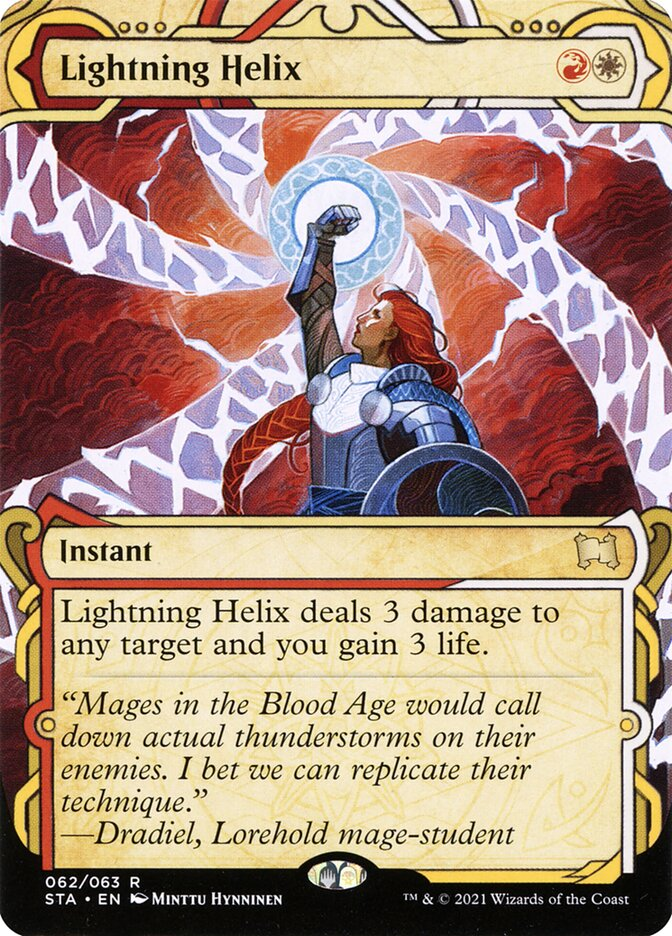
\includegraphics[width=0.6\textwidth]{Immagini/sta-62-lightning-helix.jpg}
	\caption{Carta Lightning Helix con layout Full Art}
	\label{fig:lightning_helix}
\end{figure}
La carta in se permette di infliggere 3 danni ad un qualsiasi bersaglio e di guadagnare 3 punti vita. La risoluzione dei due effetti semplici avviene contemporaneamente, ma prendendo in considerazione lo script descritto dall'Algoritmo \ref{lst:lightning_helix_fs}, si può notare come per un effetto semplice si debba creare una variabile che contenga un sotto effetto per guadagnare vita.

\begin{algorithm}
	\caption{Script della carta in Figura \ref{fig:lightning_helix} in ForgeScript}
	\label{lst:lightning_helix_fs}
	\begin{lstlisting}
Name:Lightning Helix
ManaCost:R W
Types:Instant
A:SP$ DealDamage | Cost$ R W | ValidTgts$ Any | NumDmg$ 3 | SubAbility$ DBGainLife | SpellDescription$ CARDNAME deals 3 damage to any target and you gain 3 life.
SVar:DBGainLife:DB$ GainLife | LifeAmount$ 3
Oracle:Lightning Helix deals 3 damage to any target and you gain 3 life.
	\end{lstlisting}
\end{algorithm}


\section{Lunar, un nuovo linguaggio}\label{sec:lunar_dsl}


Lunar nasce dall'idea di sviluppare un nuovo motore di regole per la gestione delle carte nei giochi di carte collezionabili, fornendo il proprio linguaggio di scripting dedicato. Si ispira alla struttura dei file YAML per rendere l'interazione con il linguaggio più accessibile e intuitiva. L'obiettivo di Lunar è risolvere le limitazioni riscontrate nell'utilizzo di ForgeScript, garantendo una maggiore leggibilità e semplificando la gestione degli effetti complessi all'interno del contesto dei giochi di carte collezionabili.


Di seguito, è presentato come potrebbe apparire la struttura di una carta  di \emph{Magic} scritta in Lunar.

\begin{algorithm}[ht]
	\caption{Struttura di una carta usando Lunar espressa in EBNF}
	\label{lst:ebnf_card}
	\begin{lstlisting}
<card> := <name> <new_line>
          <mana_cost> <new_line>
          <layout> <new_line> 
          <card_type_statement> <new_line> 
          <subtype_statement> <new_line>
          [ <supertype_statement> <new_line> ]
          [ <keywords> ]
          [ <effects> ]
          [ <oracle_text> <new_line>]
          [ <faces> <new_line>]
          [ <power> <new_line>]
          [ <toughness> <new_line>]
          [ <loyalty> <new_line>]
          [ <defence> <new_line>];
	\end{lstlisting}
\end{algorithm}
La seguente grammatica (Algorimo \ref{lst:ebnf_card}) definisce i diversi elementi che compongono una carta, come il nome, il costo di mana, il tipo di carta, le abilità, gli effetti e così via. Questa struttura fornisce una guida su come scrivere correttamente il codice di una carta usando Lunar, garantendo coerenza e uniformità nella sua definizione.
Questi elementi sono rappresentati come regole grammaticali distinte, ciascuna delle quali è seguita da una nuova riga e da un'indentazione per garantire una maggiore leggibilità .

\begin{algorithm}[ht]
	\caption{Struttura di effetto di una carta usando Lunar espressa in EBNF}
	\label{lst:ebnf_effect}
	\begin{lstlisting}
<effects> := `effects: ' <new_line>
                      effect_collection;
<keyword> := `type: ' ( `simple' 
                      | `with_amount' 
                      | `with_amount_and_type' 
                      | `with_cost' 
                      | `with_cost_and_type' 
                      | `with_cost_and_amount'
                      | `with_type' ) <new_line>
              `name: ' keyword_name new_line
              [ `cost: ' {complete_cost}+ <new_line>]
              [ `amount: ' <number> <new_line>]
              [ `affected_type: ' ( <supertype> 
                                  | <card_type> 
                                  | <subtype> ) 
                                 <new_line> ];
         
<effect_collection> :=  {<indent>}+ ( <activated_ability> 
                                    | <base_ability>
                                    | <complex_ability> ) 
                        <new_line> 
                        {effect_collection};
    \end{lstlisting}
\end{algorithm}

Successivamente, la grammatica definisce la struttura degli effetti di una carta, che possono essere di diversi tipi come abilità attivabili, abilità di base o abilità complesse. Ogni tipo di effetto è rappresentato come una raccolta di effetti, ognuno dei quali può essere composto da vari componenti come il tipo di effetto, il nome, il costo, la quantità e il tipo di carta interessata (Algorimo \ref{lst:ebnf_effect}).

Di seguito viene riportato il codice scritto in Lunar della carta in Figura \ref{fig:lightning_helix}:

\begin{algorithm}[ht]
	\caption{Script della carta in Figura \ref{fig:lightning_helix} in Lunar}
	\label{lst:lightning_helix_ln}
	\begin{lstlisting}
name: Lightning Helix
mana_cost: R W
card_type: instant
effects:
    effect:
        type: base
        mode: damage
        target: any_target
        amount: 3
    effect:
        type: base
        mode: life_gain
        target: card_owner
        amount: 3
oracle_text: <Lightning Helix deals 3 damage to any target and you gain 3 life.>
	\end{lstlisting}
\end{algorithm}




Ora proviamo a mettere a confronto come la carta ``Primeval Titan" (vista in Figura \ref{fig:one}) possa essere scritta nel linguaggio ForgeScript e Lunar.


Nel linguaggio ForgeScript, l'implementazione della carta è definita tramite una serie di specifiche riguardanti il nome, il costo di mana, il tipo di carta, le abilità e gli effetti, tutto all'interno di un formato dettagliato e strutturato. Le regole e le azioni sono espresse in modo più verboso e dettagliato, delineando chiaramente le condizioni e gli effetti associati all'entrata in gioco o all'attacco della carta ``Primeval Titan".


\begin{algorithm}
	\caption{Esempio della carta in Figura \ref{fig:one} in ForgeScript}
	\label{lst:prime_titan_fs}
	\begin{lstlisting}
Name:Primeval Titan
ManaCost:4 G G
Types:Creature Giant
PT:6/6
K:Trample
T:Mode$ ChangesZone | Origin$ Any | Destination$ Battlefield | ValidCard$ Card.Self | Execute$ TrigChange | OptionalDecider$ You | TriggerDescription$ Whenever CARDNAME enters the battlefield or attacks, you may search your library for up to two land cards, put them onto the battlefield tapped, then shuffle.
T:Mode$ Attacks | ValidCard$ Card.Self | Execute$ TrigChange | TriggerZones$ Battlefield | OptionalDecider$ You | Secondary$ True | TriggerDescription$ Whenever CARDNAME enters the battlefield or attacks, you may search your library for up to two land cards, put them onto the battlefield tapped, then shuffle.
SVar:TrigChange:DB$ ChangeZone | Origin$ Library | Destination$ Battlefield | Tapped$ True | ChangeType$ Land | ChangeNum$ 2 | ShuffleNonMandatory$ True
SVar:HasAttackEffect:TRUE
Oracle:Trample\nWhenever Primeval Titan enters the battlefield or attacks, you may search your library for up to two land cards, put them onto the battlefield tapped, then shuffle. 
	\end{lstlisting}
\end{algorithm}


\begin{algorithm}
	\caption{Esempio della carta in Figura \ref{fig:one} in Lunar}
	\label{lst:prime_titan_lunar}
	\begin{lstlisting}
name: Primeval Titan
mana_cost: 4 G G
layout: single_face 
card_type: creature
subtype: giant
keywords: 
    keyword:
        type: simple
        name: trample
effects:
    effect:
        type: trigger
        event:
            mode: change_zone
            who: self
            from: anywhere
            to: battlefield
            optional_choice: yes
            optional_decider: card_owner
        event:
            mode: attack
            who: self
            optional_choice: yes
        effect:
            type: base
            mode: move
            from: library
            to: battlefield
            target: land
            amount: 2
            how: tapped
        effect:
            base:
            mode: shuffle
            target: library
oracle_text: <Trample\nWhenever Primeval Titan enters the battlefield or attacks, you may search your library for up to two land cards, put them onto the battlefield tapped, then shuffle.>
power: 6
toughness: 6
	\end{lstlisting}
\end{algorithm}


In contrasto, l'approccio Lunar offre una sintassi più concisa e strutturata, utilizzando un formato ispirato alla leggibilità dei file YAML. La carta è definita in modo più diretto, con chiavi e valori organizzati in una struttura gerarchica. Le abilità e gli effetti sono suddivisi in modo logico, con una chiara distinzione tra eventi come l'entrata in gioco e l'attacco, e le azioni associate ad essi. Questo approccio più compatto rende il codice Lunar più leggibile e facile da comprendere per gli sviluppatori e gli utenti.

In conclusione, sebbene entrambi gli script definiscano la stessa carta, Lunar si distingue per la sua sintassi più pulita e intuitiva, che può rendere il processo di sviluppo e comprensione delle regole del gioco più efficiente e accessibile.
       


\section{QLoRa e PEFT}\label{sec:qlora_peft}



\chapter{Implementazione}\label{chapter:implementazione}
NB: CITARE HPC DI ATENEO

\section{Autotrain Advanced}\label{sec:autotrain_advanced}

\section{HPC + Autotrain}\label{sec:hpc_unipr_autotrain}

\section{HPC + Evaluation}\label{sec:hpc_unipr_evaluation}
%
%
%%%% Le Conclusioni
\pagestyle{plain}
\chapter*{Conclusione} %Se si cambia il Titolo cambiare anche la riga successiva così che appia corretto nell'conclusione
\addcontentsline{toc}{chapter}{Conclusione} %Per far apparire Introduzione nell'indice (Il nome deve rispecchiare quello del chapter)
Conclusione che riassume il lavoro svolto ed eventuali lavori futuri.


%
%%%% La bibliografia

\bibliographystyle{unsrt} %{plain} -- Scegliere lo stile preferito
\cleardoublepage
\addcontentsline{toc}{chapter}{\bibname}
\bibliography{Bibliografia}
%
\chapter*{Ringraziamenti}
TODO: scrivere i ringraziamenti
%
%
\end{document}